%  how do these entities communicate, or, more specifically, what communication paradigm is used?

% 3 types of communication paradigm:
%% inter-process communication
%% remote invocation
%% indirect communication



% Vi kører næsten kun med direct communication.
% Direct communication mellem clients og server
% Indirect når en client vil have kontakt med en anden client.
% Så snart de er "connected" bruger de direct communication med hinanden.

\subsubsection{Communication paradigms}
Inter-process and remote invocation communication will demand full synchronization between nodes which will cause unnecessary load on the network and forced idle-time. \smallskip

Indirect communication is instead preferred between clients. The clients interact with the server, which acts as the third party. This makes it possible to update their own state in the server, and get the latest known information for all other nodes on the network, without synchronizing with the individual clients directly. With the server acting as a third party that all clients communicate with through direct communication, such as \texttt{sockets} and/or \texttt{message parsing}, it creates an indirect communication network between all clients when they access processed information from the server. \smallskip

The standard client-server architecture is illustrated in \figref{fig:ClientServer}. Here clients are shown communicating directly with a server.

\begin{figure}[H]
    \centering
    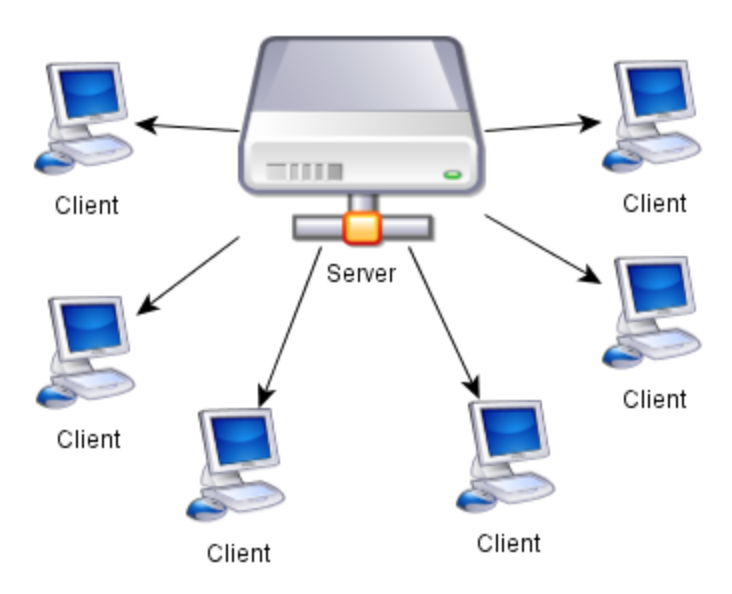
\includegraphics[width=0.5\textwidth]{images/ClientServer.png}
    \caption{Standard client-server architecture \cite{clientServerFig}}
    \label{fig:ClientServer}
\end{figure}

However the information that clients access through the server is processed and anonymized. If a client wants to know where a specific client is, the client would have to post a request to the server with that clients ID. The server would then forward that request to the other client, and if accepted, would provide each client with the others address to be used for direct communication between the two. Letting two "connected" clients communicate with direct communication instead of passing information through the server allows the clients to communicate faster, and reduces the toll put on the servers bandwidth. Like two clients can be connected directly, it is also possible to connect multiple clients as a group. The communication in a group would be carried out by multicasting messages to the entire group. Multicasting is illustrated in \figref{fig:Multicast}.


\begin{figure}[H]
    \centering
    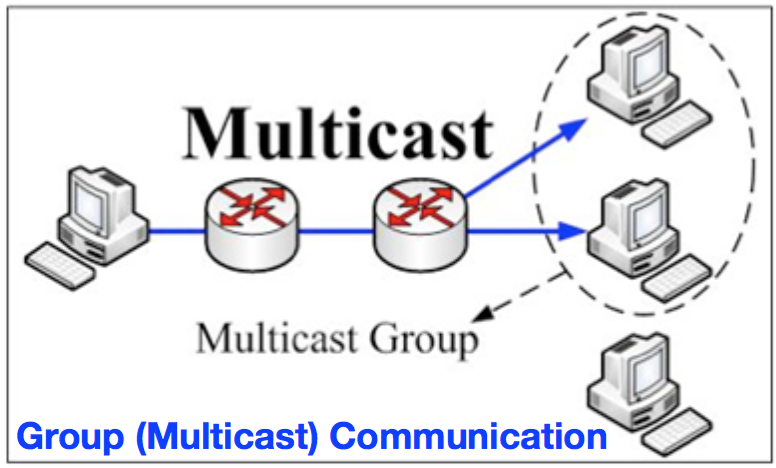
\includegraphics[width=0.6\textwidth]{images/Multicast.png}
    \caption{Illustration of multicasting a message \cite{slides}}
    \label{fig:Multicast}
\end{figure}







